\chapter{Improving Software Metrics and Refactoring}
\label{chapter:refactoring}
In Chapter \ref{chapter:problem-description}, the high amount of technical debt Tribler has accumulated over the past decade has been highlighted. We presented a history of architectural evolution and proposed a new robust and future-proof architecture in Chapter \ref{chapter:architecture}. The top-level components of of this architecture, the user interface and RESTful API, are realized and discussed in \ref{chapter:towards_new_architecture}, however, we did not focus yet on the \emph{libtribler} component, which will be the core of the Tribler platform. Readying \emph{libtribler} for the proposed architecture in Figure \ref{fig:tribler7}, requires refactoring. Since this might be the most important component in our system, we will investigate \emph{libtribler} in more detail and determine and analyse various software metrics. These metrics can provide us insights in the components of the system that are plagued with technical debt and should be refactored. A summary of the re-engineering efforts conducted during this thesis work is displayed in Table \ref{table:refactoring-summary}.\\

\begin{table}[h!]
	\centering
	\begin{tabular}{|l|l|}
		\hline
		\textbf{Lines modified} & 765 \\ \hline
		\textbf{Lines added} & 12.429 \\ \hline
		\textbf{Lines deleted (without GUI)} & 12.581 \\ \hline
		\textbf{Lines deleted (with GUI)} & 25.010 \\ \hline
	\end{tabular}
	\caption{A summary of refactoring efforts as conducted during this thesis work, excluding the work on the new user interface.}
	\label{table:refactoring-summary}
\end{table}

%\section{Software Ageing}
%We start the discussing with introducing and discussing the term \emph{software ageing}, which we think is a phenomena that is particular visible in Tribler and that helps us to find root causes of the introduction of technical debt. Software ageing is a problem in a society that is dependent on all kinds of software. The term has been coined by Dave Parnas in his talk about software ageing in 1994\cite{parnas1994software}. He points out two major reasons why software ageing is a problem. The first is the lack of movement when software fails to meet the requirements of an always-changing environment: software that users perceived as state-of-the-art several decades ago, might now be considered as legacy software, mainly due to performance reasons. For instance, where a latency of several seconds when performing a remote search in Tribler might have been acceptable several years ago, users now expect system that responds to queries within a second.\\\\
%The second reason is in particular interesting since we think this is one of the most important reasons why Tribler has evolved to the complex, hard-to-understand architecture it is today and Parnas references to this phenomena as \emph{ignorant surgery}. Changes made by people who do not understand the original design concept almost always cause the structure of the program to degrade. This is especially true for the development process of Tribler which had many contributors who are making changes to specific parts of the architecture, often ignorant about the design concepts of the original authors of the code. Moreover, some developers might not be satisfied with the implemented design and decide to change the architecture to suit their own needs, possibly leading to an even more complex system.\\\\
%There are several approaches on how we can prevent or limit the process of software ageing. The first step towards the right direction, is to think about a design that is subject to change by applying the old slogan "design for change". This slogan is reflected in the flexibility requirement of the proposed architecture in Chapter \ref{chapter:architecture}. Various design principles are helpful to prepare a system for changes such as separation of concerns and using abstractions, however, many programmers fail to correctly apply these changes in software, either due to ignorance or recklessness. We should also note that it is notoriously hard to consider and think about possible changes in the future before starting to write code. This is in particular applicable to Tribler, where often a short-term research goal should be achieved: developers are writing a piece of software that they need for obtaining experimental results. New features are often the product of a publication or research project which are most likely not scheduled when designing an architecture of Tribler. In fact, it is not even certain that new features will be added after a specific release, since Tribler is not considered a complete commercial product that should meet customer's expectations (although we should try to achieve the highest level of user satisfaction).\todo{verder reviewen}\\\\
%Design decisions taken during the development process are often not  documented. Developers fail to see the need for a proper documentation base and are proposing that the code is the documentation itself. However, this only works if you are following the structure they are using. Sometimes, it is more successful to communicate ideas on a higher-level, natural language that allows for less disambiguation. Tribler used to keep track of several design documents that describe the architecture, user interface decisions and research results, however, these documents are outdated and at the moment, there is no clear up-to-date description of the architecture. The lack of software artifacts will be discussed in more detail in Section \ref{sec:software-artifacts}.\\\\
%Parnas considers another option to limit software ageing: code reviews. For years, Tribler developers have created many new features which are not peer-reviewed by anyone, leading to a mix of different programming styles. Code reviews are an essential part in the software development process and should not be neglected.\\\\
%While prevention is a good medicine, we should define method that describe how we should deal with aged software. First of all, we can apply the methods we describe: change for design, code reviews and the construction of a proper documentation base. Modularisation of a system can be used to quicker identify components that are changing over time. When a product gets out of control, we should do a major restructuring of the product.

%\section{Influences of Python on software metrics}
%Tribler is written in: Python, an accessible, easy-to-learn language that is widely used in scientific applications. It is a high-level language, allowing one to express constructs with only a few lines of code. One of the most distinguishable properties of the language is that it is dynamically typed, which means that the type of a variable is not known at compile-time. This is in contrast to static typing, where this type is known to the compiler. The dynamic nature of the language has consequences on the way programmers are writing their code. A dangerous pitfall is that developers are making wrong assumptions about types of variables, leading to bugs that are only visible on runtime. Even then, it is not guaranteed that these kind of errors reveal themselves since they might be located inside a branch that is entered in a small amount of the application executions. Advantages of dynamic typing are apparent in testability since it is easier to mock objects during test execution.\\\\
%Dynamic typing also influences generated software metrics. While import graphs might give a good indicator of dependencies, they do not tell the whole story. In fact, there might be dependencies that are not visible in a generated import graph. These 'hidden' dependencies are often made between classes using the \emph{dependency injection} (DI) design pattern, a technique to not denote dependencies in the source code. For instance, if a class \emph{A} needs a particular service, this service is passed as parameter in a method call to \emph{A}. Dynamic typing makes it harder to capture such dependencies since almost no any information about types of attributes within a class can be determined at compile-time. The DI design pattern is very commonly used in Tribler and it is the preferred way to let components know about other components\todo{waarom is dit relevant?}.

\section{Improving the test suite}
The most fundamental way to verify the correctness of software is by having an well-designed and stable automated test suite. As pointed out in Chapter \ref{chapter:problem-description}, the current test suite is plagued with unstable and non-functional tests. We will discuss the performed work to strengthen and stabilize the test suite now. A summary of improvements made to various metrics related to the test suite during this thesis is presented in Table \ref{table:test-suite-improvements}. We notice that the number of unit tests has dramatically increased, while decreasing the average execution time per test and the total duration of the tests.

\begin{table}
	\centering
	\begin{tabular}{ l | l | l | }
		\cline{2-3} & \textbf{November '15} & \textbf{July '16}\\ \hline
		\multicolumn{1}{ |l| }{Number of unit tests} & 80 & 676\\ \hline
		\multicolumn{1}{ |l| }{Number of assertions} & 117 & 1205\\ \hline
		\multicolumn{1}{ |l| }{Number of failed runs after 10 runs} & 2 & 0 \\ \hline
		\multicolumn{1}{ |l| }{TLC/PLC ratio} & 0.06 & 0.14 \\ \hline
		\multicolumn{1}{ |l| }{Total Linux test duration on Jenkins (sec)} & 448 (7 min. 28 sec.) & 350 (5 min. 50 sec.) \\ \hline
		\multicolumn{1}{ |l| }{Average execution time per test (sec)} & 18.90 & 0.85 \\ \hline
	\end{tabular}
	\caption{A summary of improvements to the test suite between November '15 and July '16.}
	\label{table:test-suite-improvements}
\end{table}

\subsection{Identifying code smells in the tests}
As described in the work of van Deursen et al\cite{van2001refactoring}, there is a difference between refactoring test and production code in a sense that test code often has a characteristic set of code smells, originating from the way tests are structured. Before we start to make major modifications to the test suite, we present a list of code smells identified after a manual code review in the test suite of Tribler. This list is displayed in Table \ref{table:tests-code-smells} where for each code smell, we describe it and propose a solution.\\

\begin{table}
	\begin{tabularx}{\textwidth}{|X|X|X|}
		\hline
		\textbf{Code smell} & \textbf{Description} & \textbf{Solution}\\ \hline
		Dependencies on external resources & Various tests are using external resources, leading to unpredictable and unstable tests. & Remove the dependency on the resource or make sure that the resource is locally available (see Chapter \ref{subsec:external-network-resources}). \\ \hline
		State leak & The state of a previous executed test is leaking to the next test, mostly notable due to delayed calls left in the Twisted reactor after shut down. & Make sure that any delayed call in the reactor is removed when shutting down Tribler. \\ \hline
		Too much responsibility & Many tests have multiple responsibilities, testing both parts of the user interface and core components in Tribler. & Make sure that each test is only verifying one unit in the system. Also implement a separate test suite for the user interface.\\ \hline
		Tests with a high runtime & There are some tests that are taking long to complete (sometimes over 30 seconds). This can be an indicator that the test has too much responsibilities. & Identify why the test takes long to complete and shorten the runtime i.e. by splitting the larger test in smaller tests. \\ \hline
		Unclear assertions & Tests that have multiple assertions often do not annotate their assertion well with a clear and meaningful description & Add an annotation with the cause of the failure if an assertion fails so developers can pinpoint the problem quicker.\\ \hline
		Dependency on a Tribler session & Some tests are starting a complete Tribler session while only a small subset of the system is tested & Use mocking techniques to inject a mocked session or refactor the component so no session is required to test the component. \\ \hline
		Resource writing to the source code directory & Various tests are writing resources to the source code directory. They might accidentally end up in the VCS if developers are not noticing these files. & Temporary resources produced by tests should always be written to a temporary directory that is cleaned after test execution. \\ \hline
		Claiming the same local network port & Some tests that are running in parallel are claiming the same local network port, leading to test failures. & Reserve port ranges to individual parallel test runs or try to avoid the allocation of local ports. \\ \hline
		Timing issues & Various tests are asserting a condition after a fixed time interval. This interval is often based on intuition rather than empirical data. This is particularly dangerous when the test is dependent on external resources. & Refactor the test so the condition check is no longer necessary.\\ \hline
		No usage of comments & There are no comments, explaining what the the tests are testing and what the expected output is. & Comments should be added that explains the purpose of the test together with the expected in- and output. \\ \hline
		No directory structure in the test package & There is no directory structure and almost all tests are located inside the same directory. & Restructure the tests package and organise tests in different, logical named directories.\\ \hline
	\end{tabularx}
	\caption{Identified code smells in the test suite of Tribler as of November '15.}
	\label{table:tests-code-smells}
\end{table}

Table \ref{table:tests-code-smells} has been used as reference during the refactoring efforts of the test suite and in this thesis work, we fixed various of the outlined code smells. Dependencies on external resources have been reduced to a minimum as explained in Subsection \ref{subsec:external-network-resources}. The efforts on increasing the stability of the tests is outlined in Subsection \ref{subsec:instability-tests}. During the refactoring process of tests, we placed clear assertions, added comments and got rid of managing Tribler sessions as much as possible.

\subsection{Improving Code Coverage}
Code coverage is defined as the percentage of source code that is covered by at least one test in the test suite. Our continuous integration environment offers tools to track the code coverage over time. After each automated test suite execution a comprehensive report with detailed information about the code coverage is generated. The reported metrics by this report are not accurate enough since some third-party libraries are included in the coverage report, such as the VLC bindings and \emph{pymdht}, a library to fetch peers from the Distributed Hash Table (DHT). Also, the code coverage of Dispersy is included in these reports while we consider Dispersy as a separate engineering project.\\\\
The improvements in the code coverage metrics during the span of this thesis are displayed in Table \ref{table:code-coverage-table}. Branch coverage is a metric that specifies how well conditional statements are covered. This metric includes the fact that a conditional is either resolved to true or false, possibly influencing the program execution path. In the ideal scenario, we wish to have tests that cover all conditional statements in the case they resolve to \emph{true} and in the case they resolve to \emph{false} so we cover all possible execution paths in the program. This objective gets significantly harder to achieve when code with many nested conditional statements is written. The cyclomatic complexity as developed by McCabe in 1976\cite{mccabe1976complexity} is a quantitative measure of the number of linear independent paths through a program's source code. Any conditional written has a negative effect on the cyclomatic complexity.\\\\
While at first sight it may look like the code coverage has not increased significantly, we should emphasize that the complete architecture of the tests have been overhauled in parallel. Refactoring of the test suite had consequences on the code coverage in other locations in the code base. For instance, the smaller unit tests are not starting the old user interface, leading to a lower coverage in that module.\\\\
Improving the code coverage has been done by writing small unit tests where we are using mocked objects to have better control over the system we are testing. Using mocking in Tribler is a necessary since some components have many other dependencies that are hard to keep under control without using custom, controlled objects. Libtorrent is a good example of this. During this thesis, many unit tests have been written as can be seen in Figure x where the number of unit tests over time is presented. Writing tests makes a developer more aware of the written code and can be a good way to get familiar with an unknown system. Due to this, various bugs have been solved during the process of writing additional tests.

\begin{table}
	\begin{tabular}{ l | l | l | l | l | }
		\cline{2-5}
		& \multicolumn{2}{ | c | }{\textbf{November '15}} &
		\multicolumn{2}{ | c | }{\textbf{July '16} }\\
		\cline{2-5}
		& Lines coverage & Branch coverage & Lines coverage & Branch coverage\\ \hline
		\multicolumn{1}{|l|}{Core} & 71,2\% & 58,1\% & 81,2\% & 67,3\%\\ \hline
		\multicolumn{1}{|l|}{REST API} & - & - & 99,4\% & 92,7\%\\ \hline
		\multicolumn{1}{|l|}{wx GUI} & 65,8\% & 42,7\% & - & -\\ \hline
		\multicolumn{1}{|l|}{Qt GUI} & - & - & 73,4\% & 50,4\%\\ \hline
	\end{tabular}
	\caption{The difference in code coverage between November '15 and July '16.}
	\label{table:code-coverage-table}
\end{table}

\begin{figure}[h!]
	\centering
	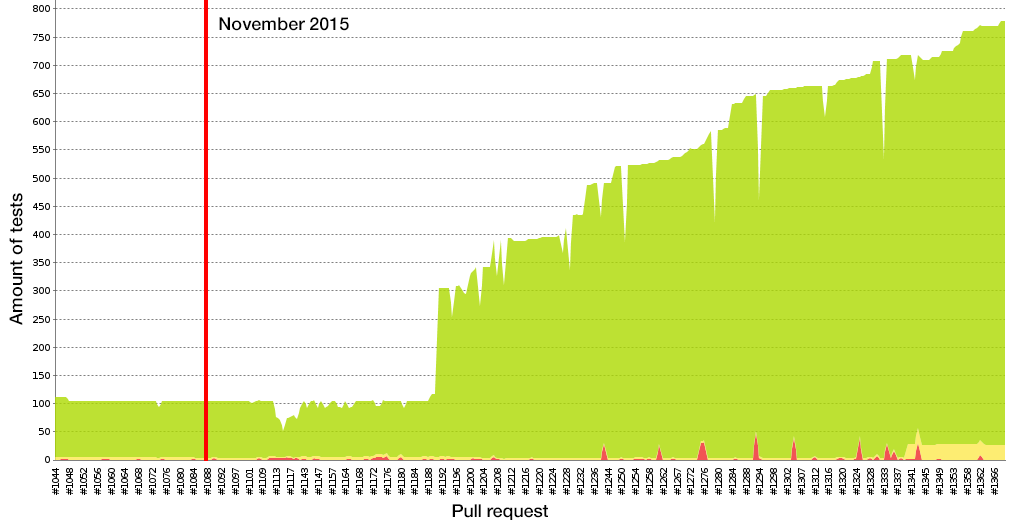
\includegraphics[width=0.8\columnwidth]{images/improving_qa/test_trend}
	\caption{The number of tests over time until July 2016 (November 2015 is annotated).}
	\label{fig:importgraph-qt-gui}
\end{figure}

In Chapter \ref{chapter:problem-description}, Figure \ref{fig:tests-ratio-tribler} we presented the ratio between the number of code lines in the tests package and the amount of other code lines over time. Together with the code coverage, this number can be a useful metric to developers. While one might argue that having a high code coverage in conjunction with a low TLC/PLC ratio is a desired result, it indicates that the tests are not granular enough and are actually doing many different operations. A low code coverage with a high TLC/PLC ratio indicates that there are some flaws in the tests, possibly that they are testing the wrong components of the system. In the case of Tribler, the coverage is reasonable (still a bit low) but the TLC/PLC ratio is very low, indicating that most likely, the tests are not granular enough.\\\\
After writing additional unit tests, removal of the old user interface and addition of the new one, the new ratio is \emph{0.16} which means that there is roughly one line of test code for six lines of other source code in Tribler. Defining a good TLC/PLC ratio is dependent on the used programming language, development methodology and application structure. Discussion on the wiki of Ward Cunningham\cite{c2tlcratio} proposes an optional ratio of 1:1, however, several other ratios have been proposed on the same page such as 2:1 and 5:1. In the work described in \cite{van2001refactoring}, an ideal ratio of 1:1 is proposed. Overall, the trend seems to be that the amount of test line code is around the same or a bit higher than the lines of production code. An important question is whether this proposed ratio also holds for Tribler. Tribler differs from a commercial software engineering project in the sense that it is used for scientific research. When performing research, it is easy to ignore testing and focus on the results that are gathered by the system. The difficulty here is that Tribler is distributed and used by over a million of users, requiring at least some form of quality assurance. We think a better optional TLC/PLC ratio for the Tribler project might be 1:2.\\\\
To make sure that the responsibility of code coverage is not neglected in future work on Tribler, an addition check for each pull request has been added that verifies that the code contributed in the respective pull request is covered by tests. While not created by the author of this thesis, this check is an effective way to keep the code coverage metric under control.

\subsection{Testing the New User Interface}
One of the issues in the old testing framework, was that there is no clear separation between tests that are testing the user interface and tests that are testing core functionalities of Tribler. This is one of the reasons that have led to big, extensive tests in the old test suite. Since testing is an important aspect of this thesis work, writing proper tests for the user interface has been a prioritized task earlier in the development process of the new user interface.\\\\
GUI testing is an interesting area in the field of software engineering and is part of the application testing methodology. GUI testing can also be more involving than unit testing since a user interface might have many different operations and verification of the correct output of an action is often a non-trivial task. A popular way of testing user interfaces is a Finite State Machine-based modelling where the user interface is modelled as a state machine that transitions when actions in the user interface are performed\cite{clarke1998automated}\cite{belli2001finite}. Another model to create a test script based on a genetic algorithms has been proposed by the work of Kasik et al\cite{kasik1996toward}.\\\\
We started out by removing the \emph{wxPython} dependency from the test suite by making sure that no test is starting a user interface. Preferably, we want to avoid starting a headless Tribler session, however, for some situations this requires too much refactoring, for instance, when testing the tunnel community that facilitates anonymous downloading and seeding.\\\\
Testing the new Qt user interface makes use of the \emph{QTest} framework. This framework provides various tools to perform non-blocking waits and to  simulate mouse clicks and keyboard actions. A sample of a test written with the \emph{QTest} framework is illustrated in Listing \ref{lst:qtest-sample}. After the interface is started, the test navigates to the home page, clicks on the \emph{channels} tab button and waits for items to be loaded. During the test execution, two screenshots are captured, one when we are loading items and another one when the requested items are loaded and displayed.\\\\
Primitives to capture screenshots during test execution has already been implemented and used in the old test suite, using the rendering engine of \emph{wxPython}. The \emph{Qt} frameworks offers similar tools. Captured screenshots are exported to \emph{jpg} files under a name specified by the developer. In the sample given in Listing \ref{lst:qtest-sample}, the exported screenshots are saved as \emph{screenshot\_home\_page\_channels\_loading.jpg} and \emph{screenshot\_home\_page\_channels.jpg} respectively. At the end of each test run, an image gallery is generated where the generated screenshots are archived and displayed in a grid. This allows developers to manually verify whether visual elements are correctly displayed. A part of the generated image gallery is displayed in Figure \ref{fig:jenkins-gallery}.

\begin{figure}[h!]
	\centering
	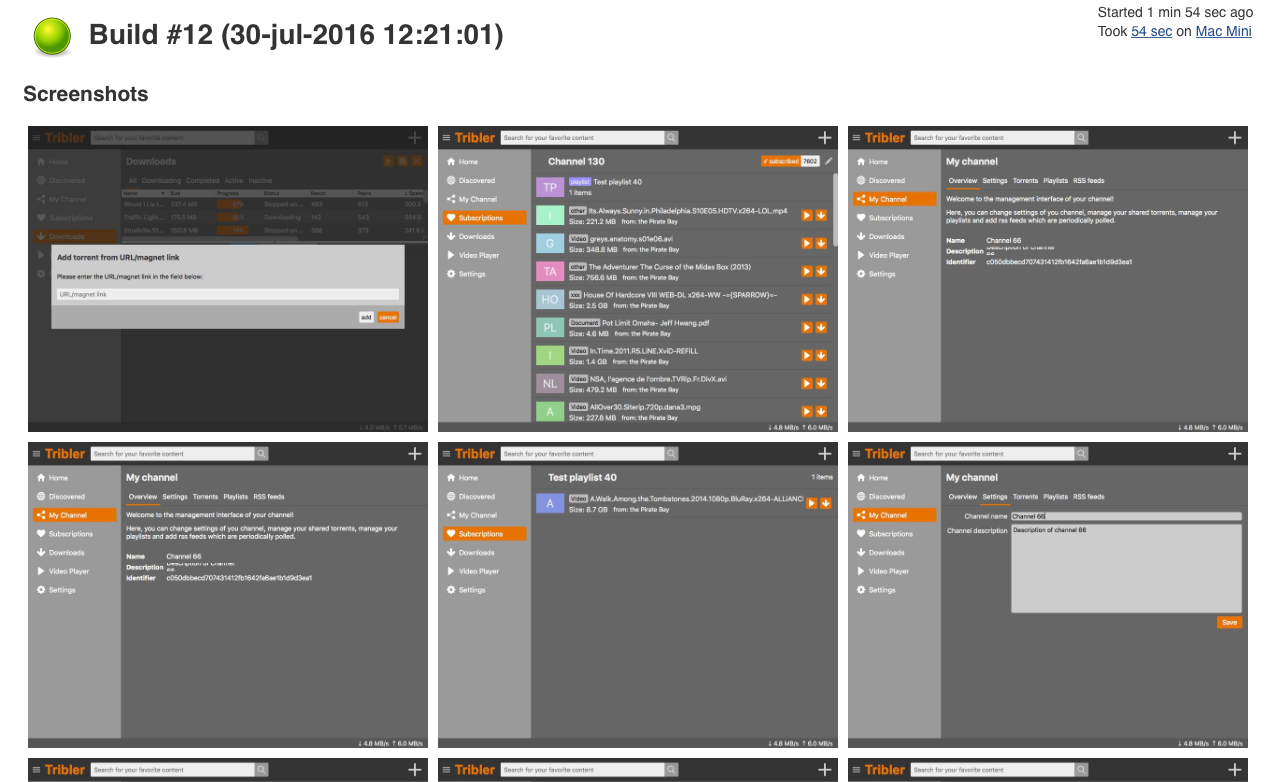
\includegraphics[width=1.0\columnwidth]{images/improving_qa/gallery_jenkins}
	\caption{The generated image gallery after executing of the user interface tests, generated by Jenkins.}
	\label{fig:jenkins-gallery}
\end{figure}

To avoid dependencies on Tribler itself and thus re-introducing the problem we are trying to solve, we created a small piece of software that provides the same interface as the REST API implemented. This 'fake' API is much simpler in nature and has a very simplistic in-memory data model. The downside of this approach is that new endpoints have to be written twice, once in Tribler and once in this fake API, providing that the new endpoint will covered by a user interface test.

\begin{lstlisting}[caption={A sample of a test that tests the new Qt Tribler GUI.},label={lst:qtest-sample}]
def test_home_page_channels(self):
	QTest.mouseClick(window.left_menu_button_home, Qt.LeftButton)
	QTest.mouseClick(window.home_tab_channels_button, Qt.LeftButton)
	self.screenshot(window, name="home_page_channels_loading")
	self.wait_for_home_page_table_populated()
	self.screenshot(window, name="home_page_channels")
\end{lstlisting}

\subsection{External Network Resources}
\label{subsec:external-network-resources}
On of the problems with the test suite was that dependencies on external network resources should either be removed or one should verify that the resources are under the control of the developer and always available. The test suite contains various tests where external torrent files are fetched from the internet, in particular, from the Ubuntu repository. While this repository can guarantee high availability, any downtime in this external resource can lead to failing tests. The implemented solution for this design flaw is to start up a local HTTP server that serves the torrent file. While this approach requires more code to manage this local server, it completely removes the dependency on the Ubuntu repository.\\\\
The same solution has been applied to solve the dependency on external seeders. A small number of tests makes assumptions on the availability of torrent pieces of the network. This certainly makes tests fail if the executing machines has a bad or even no internet connection. The process of setting up a local seeder session is straightforward. Again, this approach requires code to properly start and shut down the seeder session. The implementation is reusable to an extend that developers of tests can reuse the implemented solutions with only a few lines of code.\\\\
Unfortunately, there are some external network dependencies left which are considered harder to refactor. A handful of tests are performing a remote keyword search, requiring various communities in Dispersy to be loaded. These tests are dependent on available peers in the respective community in order to make sure there are incoming search results. The proposed solution here is to start various dedicated Dispersy sessions on the local machine. Due to time constraints, the implementation of this solution is considered future work.

\subsection{Instability of Tests}
\label{subsec:instability-tests}
A non-functional testing suite has a direct impact on the productivity of developers: when unit tests fails to reasons unrelated to the code that the developer contributed in a specific pull request, developers have to run the test suite again by placing a comment on the Pull Request that says \emph{retest this please}. Every retest operation is "wasting" several minutes since developers have to wait this time before their Pull Request can be merged and before they have the necessary feedback on the stability of their pull request. This is a structural problems that Tribler developers are experiencing since the utilization of continuous integration.\\\\
To estimate the total time developers had to wait for retests, we've written a small script that that uses the GitHub API to analyse every opened pull request and count the number of retests required. Before we present the results, we should not that we might miss some occurrences since they might have been removed. In addition, some retests might be related to failures in the continuous integration environment. In total, we counted 2045 retests in 1481 pull requests, on average, 1.38 retests for each pull request. If we use an optimistic estimation of a duration of six minutes for the execution of the full test suite, we spent around 204 hours in total retesting pull requests. We argue that we can stabilize the test suite in much less time so we need no retests anymore. To demonstrate that we are dealing with a structural problem here, the number of retests over time has been displayed in Figure \ref{fig:retest-this-please-required}.\\

\begin{figure}[h!]
	\centering
	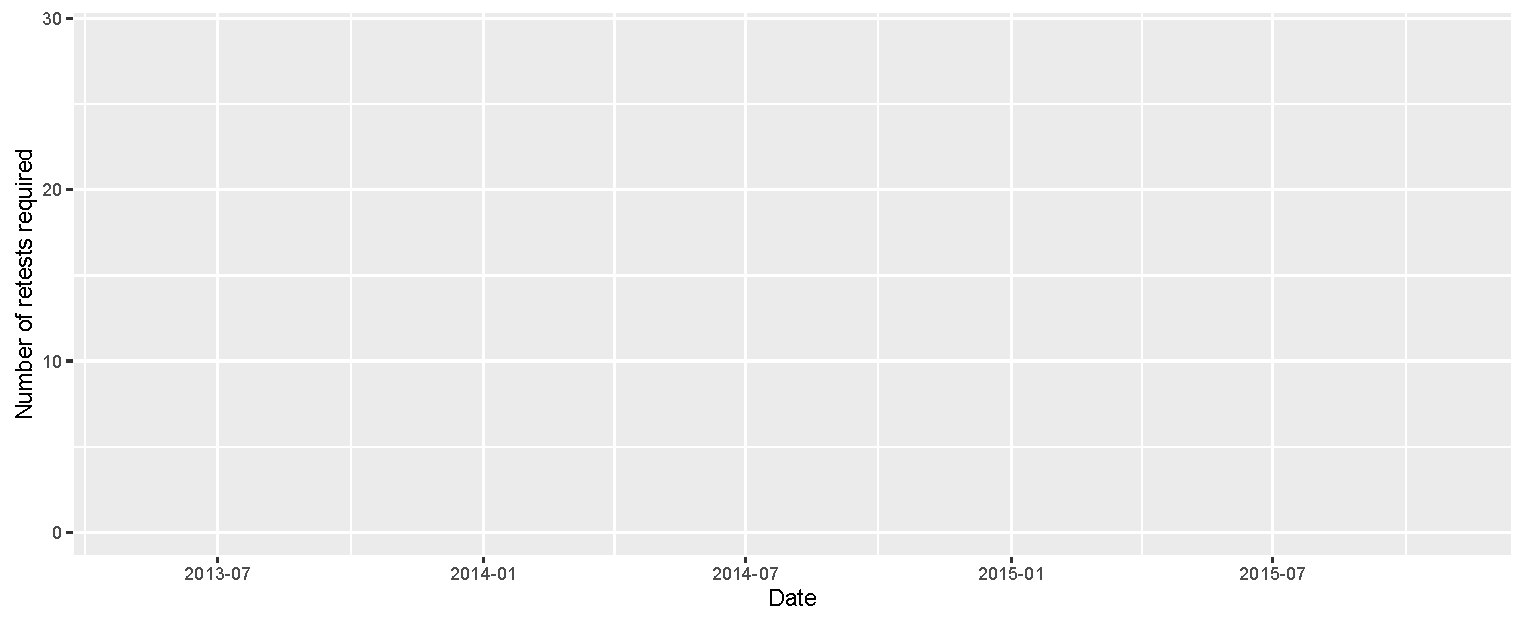
\includegraphics[width=1.0\columnwidth]{images/improving_qa/retests_required}
	\caption{The number of retests required in Pull Requests over time.}
	\label{fig:retest-this-please-required}
\end{figure}

Essentially, we are dealing here with a special kind of technical debt. Developers prudently made the decision to postpone fixing of the problem by retesting the pull request until the tests passes. The incentives to spent some time to fix errors in tests are not apparent and often, developers do not feel that they are responsible for failing tests since it might have been caused by code written by other developers. This makes it attractive to ignore test failures.\\\\
Well-designed tests should only fail if some new code is breaking existing functionality. If no changes are presents, the tests should always succeed. Reducing dependencies on external network is not sufficient to guarantee this condition in Tribler. The structural problem of the tests is that the system is infested with race conditions. Race conditions can be invisible since they often occur in a very specific runtime setting of the system, making the debugging process of these kind of errors frustrating. In fact, it is very easy to deliberately introduce a race conditions that is not noticed after the code is merged into the main branch. A complex architecture and threading model is an important asset in this process.\\\\
During this thesis, various race conditions have been detected and solved. One interesting observation is that some issues only occurred on a specific platform. We believe can be explained by differences in the implementation of underlying threading model across operating systems. The most common cause of failing tests can be addressed to delayed calls in the Twisted reactor. During the test execution, Tribler is restarted many times. If a developer leaves by accident a delayed call behind when the shut down procedure has been completed, this delayed call might be executed in the wrong Tribler session, possibly leading to an inconsistent state of the system. Making sure the reactor is completely clean is not straightforward: if one is not aware of scheduled calls in the system, the mistake is easily made.\\\\
Writing stable tests also requires the test to be limited in what they do. Each test should only be focussed on the specific part of the system that has to be tested. While often unnecessary, a significant amount of the available tests are focused on starting a complete Tribler session, testing a small subset of the system, and shutting down Tribler again. While this approach is relatively easy to code, starting a fully-fledged session often leads to more instability and unexpected side-effects during test execution. Instead, only the classes to be tested should be instantiated and any dependencies this class have, should be mocked. Mocking ensures that developers have control over dependencies, allowing them to specify any expected return value. Moreover, the execution time of these small unit tests is significantly lower than the tests where a Tribler session is managed. The additional unit tests that have been written during this thesis, are following the described design.

\subsection{Continuous Integration Enhancements}
Tribler makes use of the popular continuous integration (CI) platform Jenkins. Jenkins allows developers to define jobs which can be executed manually or when pushing a commit on the code base. This continuous integration platform is responsible for running the tests, packaging Tribler and running research-oriented experiments.\\\\
When we focus on the execution of the tests, it is immediately noticed that they are only executed in a Linux environment. Beller et al\cite{beller2016oops} conducted research on CI adoption and usage and it turned out that for some languages, it might benefit to run tests in different environment. An addition argument for this is the usage of many platform-specific workarounds we are using in Tribler. To make sure that these statements are covered, we must run the tests in this environment. This will allow developers to detect defects on other platforms more earlier in the development process. By aggregating the generated coverage report on each platform, this multi-platform setup should benefit the code coverage.\\\\
The setup of the testing environments on Windows and OS X is straightforward. New slave nodes to specify the Windows and OS X test runners have been created. The tests on OS X are executed on a Mac Mini, late 2014 model with 4GB of DDR3 memory and an Intel Core I5 1.4 GHz processor. In order to run the tests on Windows, two virtual machines using Proxmox have been created, both 32-bit and 64-bit environments. In total, the tests are executed on four platforms now: Linux, Windows 32-bit, Windows 64-bit and OS X. So far, the OS X and Windows test executers have completed over 2.500 test runs. Each test runner generates a coverage reports and these reports are merged in the final analyse step in the build pipeline.\\\\
While this is certainly a step in the right direction, there are various additional steps in the execution plan that can be performed. In Figure \ref{fig:jenkins-pipeline}, the ideal test execution plan is displayed, together with the various stages in this pipeline. We start by executing the tests on multiple platforms where during these runs, the code coverage is being tracked. After this phase, the coverage reports are combined and the total difference with the upstream branch is determined. When the commit decreases the total code coverage, the job fails.\\

\begin{figure}[h!]
	\centering
	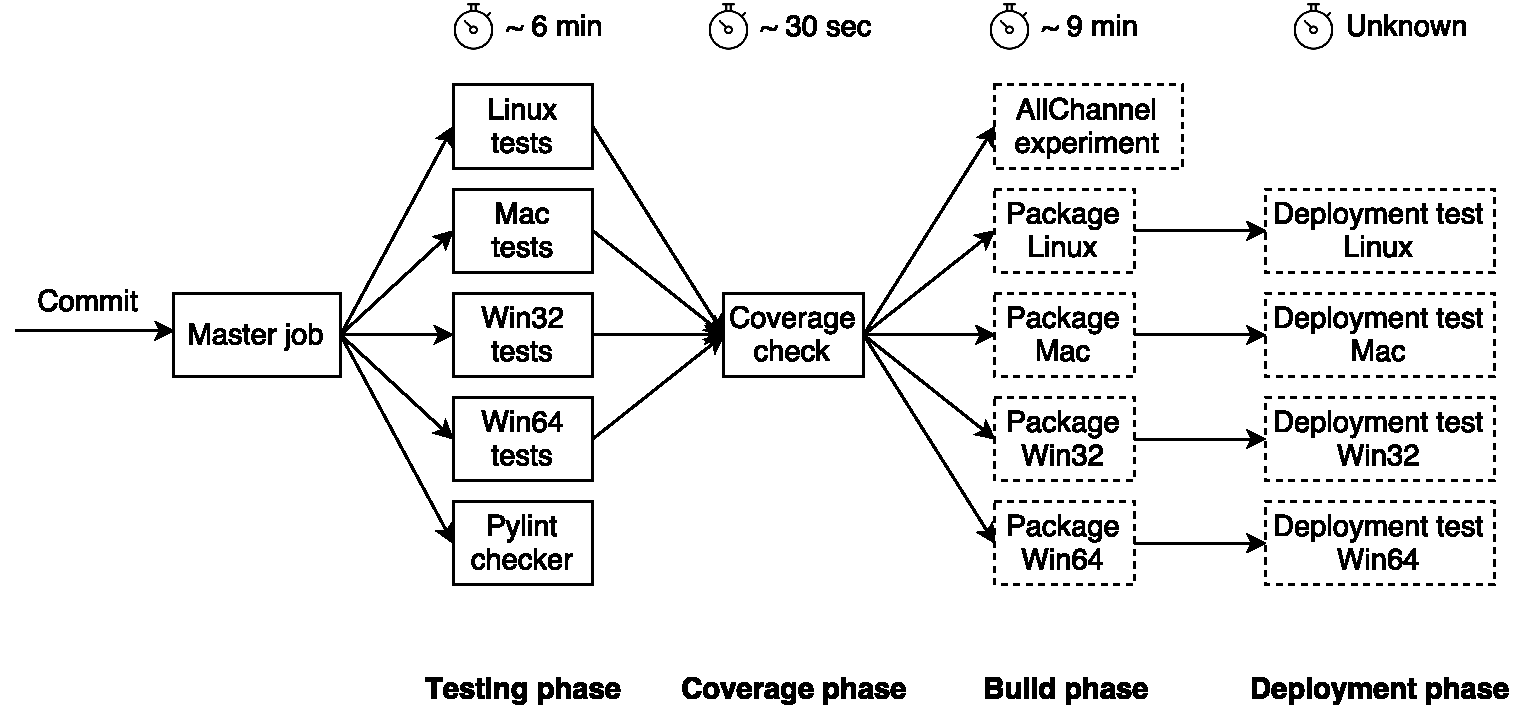
\includegraphics[width=0.9\columnwidth]{images/improving_qa/jenkins_pipeline}
	\caption{The desired test execution plan in our continuous integration environment. Dashed boxes are not implemented yet.}
	\label{fig:jenkins-pipeline}
\end{figure}

A static Pylint checker has been available to check for code style violations, however this only gave insight in the total amount of Pylint errors and did not stimulate to actually fix errors in the committed code. While not implemented by the author of this thesis, the Pylint checker has been extended to fail if new violations are introduced in the committed code. Additionally, a report is generated with an overview of the introduced violations. This helps developers to get more aware of the code style. This checker is ran in parallel with the tests to decrease the total time of the pipeline execution.\\\\
After the coverage phase has passed, jobs to package Tribler for distribution should be added. In parallel, the \emph{AllChannel} experiment can be executed. This experiment is executed on the DAS5 supercomputer and starts 1.000 Tribler clients that are synchronizing torrents and channels with each other. When the experiment is completed, several graphs are generated, providing developers insights in the consequences of their modified code when Tribler runs in a more comprehensive environment. For instance, the experiment can highlight issues in the message synchronization between peers in the network.\\\\
In parallel with the \emph{AllChannel} experiment, we can package Tribler for distribution to end-users. On Windows, an installer will be created that installs Tribler to the \emph{Program Files}. On OS X, we create a \emph{DMG} file that contains an app bundle. On Linux, the required files are bundled in a \emph{deb} archive. All these jobs can be executed in parallel. Finally, we should test whether the final distributions are working. This should be achieved by executing the final Tribler executable. A small test suite that makes use of the REST API can be created.

\section{Breaking dependencies}
As indicated by Figure \ref{fig:wx-import-graph}, Tribler is plagued with many dependencies that are leading to a highly coupled system where it is hard to reuse individual components. This Section will focus on identification and removal of undesired dependencies between packages.

\begin{figure}[h!]
	\centering
	\begin{subfigure}{.5\textwidth}
		\centering
		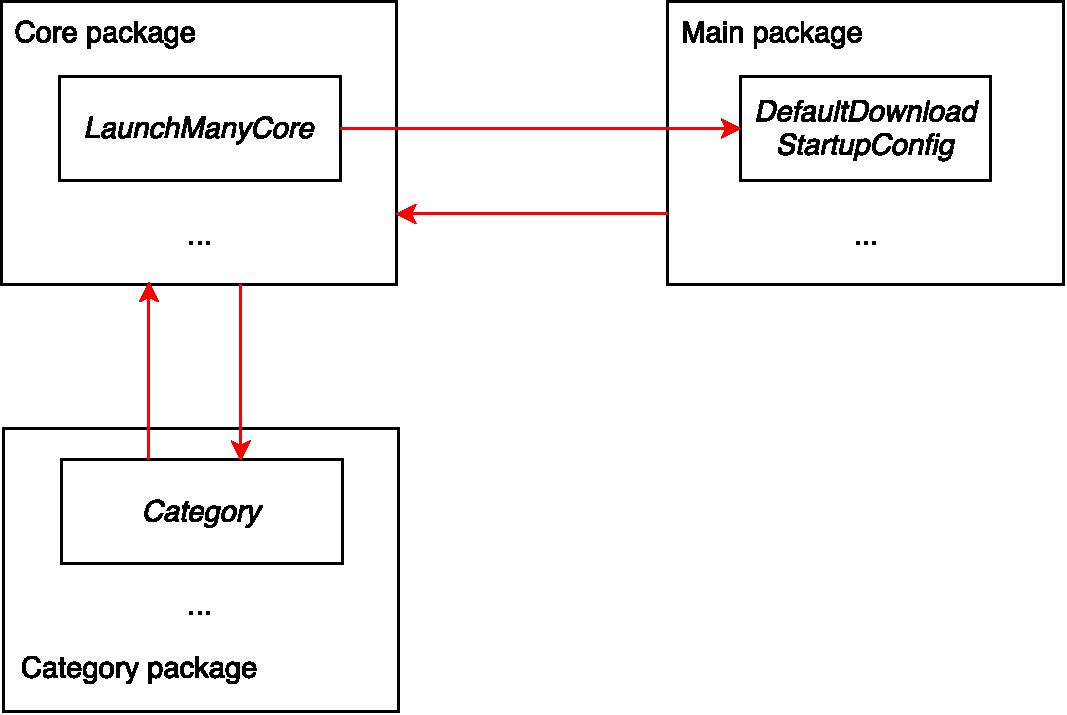
\includegraphics[width=0.9\linewidth]{images/improving_qa/cycle_tribler_package}
		\caption{Before refactoring}
		\label{fig:tribler-packages-refactoring-before}
	\end{subfigure}%
	\begin{subfigure}{.5\textwidth}
		\centering
		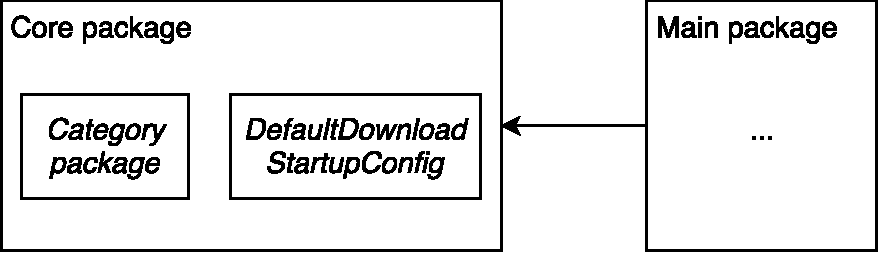
\includegraphics[width=0.9\linewidth]{images/improving_qa/cycle_tribler_package_after}
		\caption{After refactoring}
		\label{fig:tribler-packages-refactoring-after}
	\end{subfigure}
	\caption{The dependencies between Tribler modules at the highest level.}
	\label{fig:tribler-packages-refactor}
\end{figure}

\subsection{GUI and core packages}
As described in Chapter \ref{chapter:problem-description}, the source code for the user interface and Tribler core code is interleaved to a large extent and there is no clear separation between these components. There are various instances where we identified code present in the user interface code base that should be moved to the core and vice versa. To realise a clear separation between \emph{libtribler} and the user interface, we should make sure that we move code to the modules where it belongs.\\\\
In the present code base, the \emph{Core} package is dependent on the user interface which is a situation we wish to avoid since it influences the reusability and testability. The exact dependency is visible in Figure \ref{fig:cycle-main-core} and is caused by the \emph{DefaultDownloadStartupConfig} class which is located in the \emph{globals.py} file, part of the user interface module. This class is responsible for getting default configuration options when a download is being started, in case the user did not override the default options, such as destination of the downloaded file and the amount of anonymous hops used. Since the superclass of \emph{DefaultDownloadStartupConfig}, \emph{DownloadStartupConfig}, is already located in the Tribler core, the easiest solution is to move the \emph{DefaultDownloadStartupConfig} class to the \emph{DownloadConfig.py} file, which already contains the \emph{DownloadStartupConfig} class. After we moved this class to the core and modified the references to point to the new location of the class, the core is completely independent of the user interface.\\\\
The final result of the refactoring effort described above is displayed in Figure \ref{fig:tribler-packages-refactoring-after}. We readied the Main package for removal when the new user interface is ready for deployment.

\subsection{Category package}
Referring to Figure \ref{fig:tribler-packages-refactor}, we note a cyclic dependency between the \emph{Core} and \emph{Category} package. The \emph{Category} package hosts the source code to facilitate the family filter. Obviously, the family filter is used by the Tribler core, however, the family filter also has dependencies on classes inside the Tribler core, causing a cyclic dependency.\\\\
In the architecture proposed in Figure \ref{fig:tribler7}, we specified the family filter as component of libtribler. We think that the best solution to solve this dependency, is to refactor the \emph{Category} package inside the Core package so it's part of libtribler. This change is reflected in Figure \ref{fig:tribler-packages-refactoring-after}.

\subsection{Video Player}
We will now focus on the core package which contains some code that should not be present. The most obvious piece of user interface-related code is attributed to the (embedded) video player in Tribler which is handled by the \emph{VideoPlayer} class in the \emph{Video} package. This class makes use of the VLC bindings for Python, however, in our design, the core does not need to have any dependency on VLC since managing the video player is a operation that should be performed on the level of the user interface. Figure \ref{fig:video-package-refactoring-before} shows the import graph of the  \emph{Video} package before refactoring. The \emph{LaunchManyCore} class contains code to initialize all components available in Tribler, including the \emph{VideoPlayer}. When initializing, this \emph{VideoPlayer} creates a \emph{VideoServer} that is responsible for the streaming capabilities of Tribler. The \emph{VLCWrapper} class contains various utility methods to work with raw VLC data such as the time position within a video.\\\\
We performed some refactoring work on this package and removed the \emph{VideoServer} and \emph{VLCWrapper} classes. The composition of the \emph{Video} package after this operation is displayed in Figure \ref{fig:video-package-refactoring-after}. We modified the code such that \emph{LaunchManyCore} the starts a video server instead of a video player. We note that there are some classes that appears to be unused, such as \emph{VideoUtility} and \emph{utils}: these classes contains some helper methods to retrieve thumbnail images from a video file. Due to time constraints, we are unable to implement these features in the new user interface so we keep these files as reference for future development.

\begin{figure}
	\centering
	\begin{subfigure}{.5\textwidth}
		\centering
		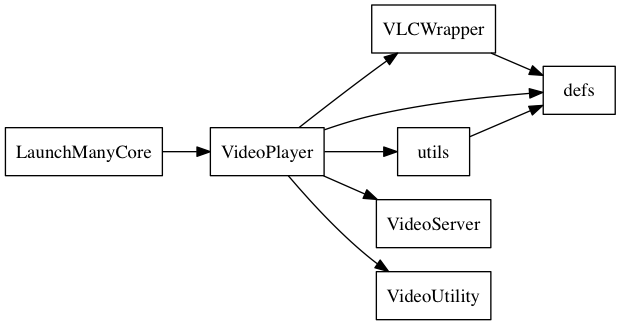
\includegraphics[width=.9\linewidth]{images/implementation/output_video_nov15}
		\caption{Before refactoring}
		\label{fig:video-package-refactoring-before}
	\end{subfigure}%
	\begin{subfigure}{.5\textwidth}
		\centering
		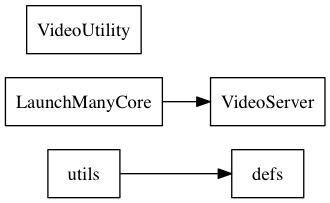
\includegraphics[width=.7\linewidth]{images/implementation/output_video_july16}
		\caption{After refactoring}
		\label{fig:video-package-refactoring-after}
	\end{subfigure}
	\caption{The import graph of the \emph{Video} package in the Tribler core before and after refactoring.}
	\label{fig:video-package-refactoring}
\end{figure}

\section{Updating software dependencies}
A cause of ageing software is the inability of developers to adopt to changing environment. This might be addressed to adoption of dependencies in the past, dependencies that are not maintained any more at a point in the future. Replacing these dependencies might be a non-trivial programming task, requiring the programmer to get familiar with both the interface of the old and new dependency.\\\\
Tribler has a long list of dependencies, both in the code base and dependencies that are used for software packaging and testing. Keeping these dependencies on the latest version is often neglected or overlooked. Sometimes, this is not even possible, due to missing software in package managers such as \emph{yum}, the package manager used by CentOS or \emph{apt}, the package manager of Debian and Ubuntu. While this restriction holds for operating systems where we are not packaging dependencies, we have the freedom to package any dependency we want on Windows and MacOS so preferably, we often want to ship the latest, stable release of a dependency in our Tribler distribution.\\\\
During this thesis, we updated several dependencies to newer versions, most notably \emph{libtorrent}. The code to handle the communication with this library (located in the \emph{Libtorrent} package) contained calls to deprecated functions in the \emph{libtorrent} library, functions that are not guaranteed to be maintained or compatible. We identified these calls as follows: first, a version of \emph{libtorrent} has been compiled without deprecated methods and assertions. Next, we manually ran Tribler and the test suite, observing any crash due to libtorrent. In total, this method yielded seven calls to deprecated methods that have been updated to call the correct function. Not only deprecated calls have been removed, we also fixed various assertions that were triggering due to incorrect assumptions made in the code. In order to remain backwards-compatible with older version of the libtorrent library (that some Ubuntu or Debian users might have installed on their system), some checks in the Tribler code base had to be implemented to check for the presence of a particular method in libtorrent.\\\\
An additional outdated dependency in Tribler is \emph{py2exe}, used to create a Windows executable file out of the source code. \emph{py2exe} performs a static code analysis and determines code dependencies that should be bundled in the executable. Unfortunately, the library has not been updated since 2014 and requires a significant amount of code to make sure that everything works when Tribler is packaged and archived. We made attempts to replace \emph{py2exe} with the more mature, well-maintained \emph{PyInstaller} that also offers support for \emph{PyQt5}, the framework used for creation of the new interface. This library is not only easier to use, it also works across multiple platforms, allowing us to also drop the \emph{py2app} dependency which is used to distribute Tribler on MacOS. While not ready for deployment yet, a proof-of-concept has been created that successfully packages Tribler together with the new user interface into Windows and MacOS executable files. Further work should focus on the removal of \emph{py2exe} and \emph{py2app} in favour of \emph{PyInstaller}.

\section{Improving Sofware Artifacts}
\label{sec:software-artifacts}
During the last ten years of development on Tribler, the main focus of the project has been to deliver working code. The project has a severe lack of maintained software artifacts, including documentation, comments and architectural diagrams, leading to a huge amount of \emph{documentation debt}. Most of the conducted research was documented on the Tribler wiki\footnote{https://www.tribler.org/TitleIndex/}, however, this wiki is very outdated and not maintained anymore. After the migration of the project to GitHub, this platform was favoured over continued usage of the Tribler wiki archive.\\\\
At the moment, there are several distinct locations where we store the few software artifacts we have. Documentation is either stored in the GitHub wiki or in the `docs` directory in the Tribler source code. The ideal situation is to have one single, useful location for all generated documents during the process. Many Python projects are using \emph{readthedocs}, a platform to host documentation for free. The hosted documentation should be located in the Tribler repository, in \emph{reStructuredText} (RST) format. By using the Python module Sphinx, a HTML website can be generated from all the available documentation. Sphinx also provides tool for localization of documentation.\\

\begin{figure}[h!]
	\centering
	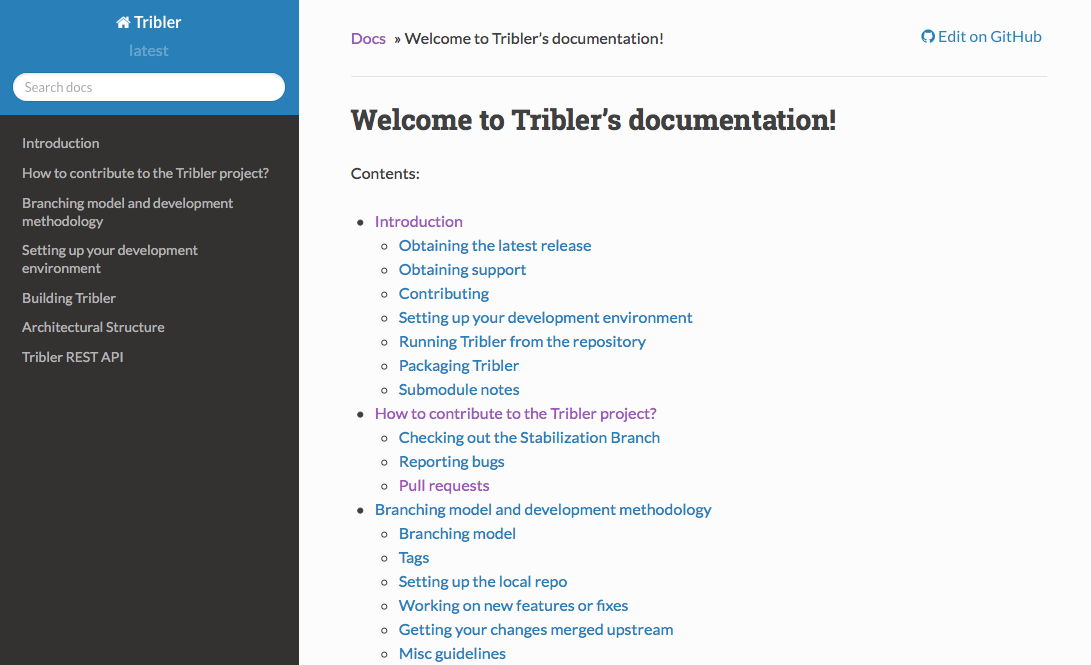
\includegraphics[width=1.0\columnwidth]{images/improving_qa/readthedocs}
	\caption{The documentation of Tribler, as displayed on the \emph{readthedocs} website.}
	\label{fig:old-threading-model}
\end{figure}

During this thesis, all available documentation of Tribler has been rewritten to make use of RST in conjunction with \emph{Sphinx}. Moreover, the available documentation has been improved with several guides, in particular, guides that help users to create a developer environment on their machine. Prior, these guides were not available and development on other platforms than Linux was not supported. By the addition of these guides, new developers can start as soon as possible with development on Tribler.\\\\
The REST API in particular has been very well documented. Since external developers can use the REST API to control Tribler, we wish to provide a clear and comprehensive documentation base for this API. To simplify the process of writing documentation, the documentation can be written as doc strings above each method. The \emph{autosummary} tool that is executed each time the documentation is built, navigates through the API code base, extracts all doc strings and generates page sections for each documented method. The doc string can also be attributed with \emph{RST} syntax. This feature decreases chances that developers accidentally forget to write documentation since the code and documentation is present in the same file instead of being spread across different files.

\section{Preventing Technical Debt}
Prevention is the best medicine and we should think about the prevention of technical debt in future development stages. Tribler needs a culture change regarding technical debt: developers have never been aware of the long-term consequences of the Tribler architecture and their work. To stop the deterioration of the system, new developers need to be come aware of the term technical debt and the term needs to play a bigger role when making longer-term decisions. In addition, we present the following list of preventions:
\begin{itemize}
	\item Code reviews is an effective way of ensuring that problems in the code are detected as early as possible\cite{18fpreventdebt} but additionally, it helps developers to learn from their mistakes. The new policy introduced during this thesis requires each pull request of developers to be at least reviewed by two other Tribler developers. This policy also helps developers to get aware of ongoing projects that other developers are working on.
	\item Continuous integration and automated testing is an excellent opportunity to maintain a high level of code quality and to catch bugs during the development process before customers report them. The work as described in this Chapter, has matured the CI and testing environment so it can be used reliably by the next generation of Tribler developers.
	\item Our CI environment already used static analysis tools to report violations in the source code which is an effective way to make developers aware of their introduced violations\cite{nagappan2005static}. However, this tool has been implemented as separate job and is not executed on every pull request. This has been changed so developers receive fast feedback when they push a new commit to GitHub. The implemented checks for every pull request are visible in Figure \ref{fig:jenkins-check}. Besides the reports of the test execution on multiple platforms and the code violation reporter, the code coverage report fails if developers added or modified lines that are not covered by a test. This tool will definitely contributes towards an increase of the code coverage metric.
\end{itemize}

\begin{figure}[h!]
	\centering
	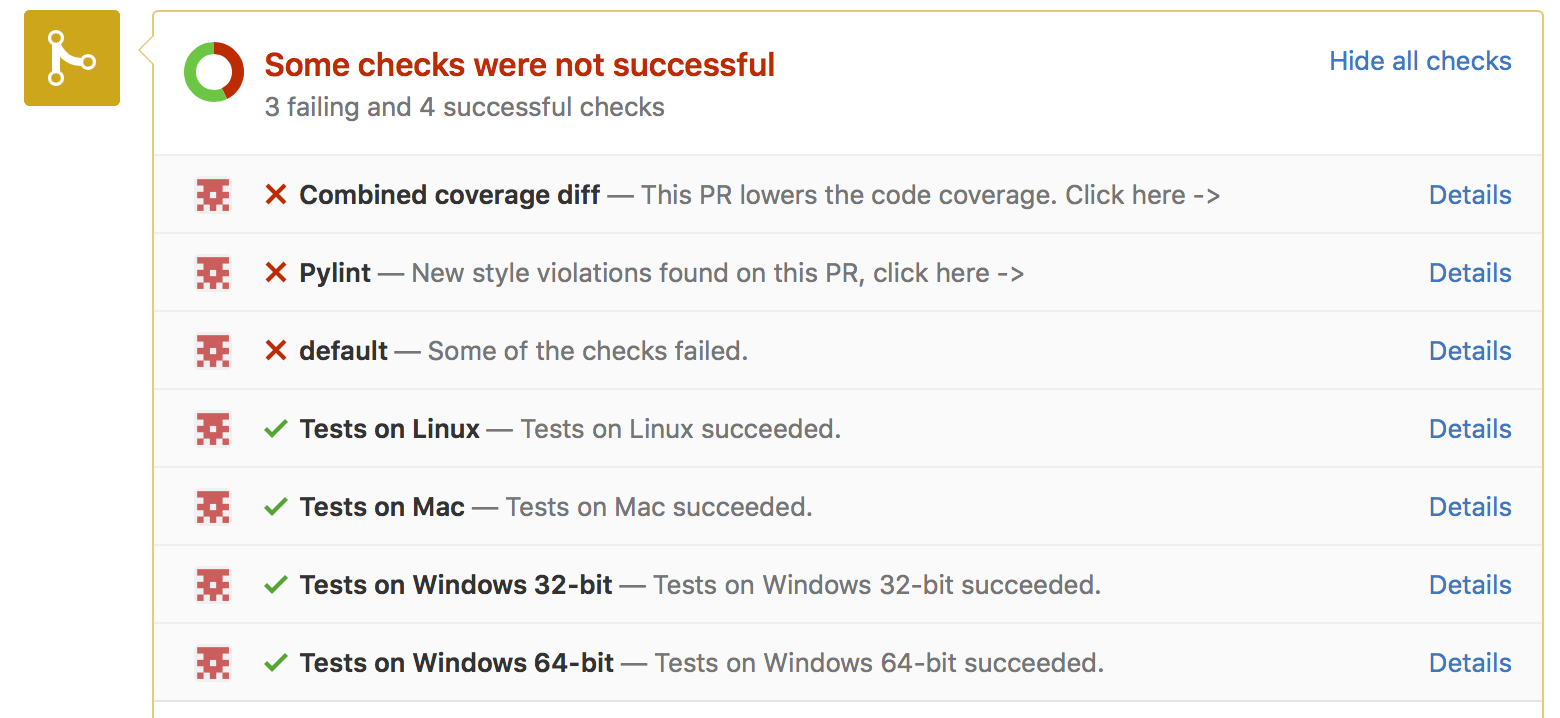
\includegraphics[width=1.0\columnwidth]{images/improving_qa/jenkins_checks}
	\caption{The implemented checks in Jenkins, executed on every new commit in a pull request.}
	\label{fig:jenkins-check}
\end{figure}